\documentclass[12pt, a4paper]{article}
% Some fancy symbols
\usepackage{textcomp}
\usepackage{stmaryrd}
\usepackage{cancel}

% Some fancy symbols
\usepackage{textcomp}
\usepackage{stmaryrd}


\usepackage{array}

% Math packages
\usepackage{amsmath,amsthm,amssymb, amsfonts, mathrsfs, dsfont, mathtools}
% \usepackage{mathtext}

\usepackage[bb=boondox]{mathalfa}
\usepackage{bm}

% To conrol figures:
\usepackage{subfig}
\usepackage{adjustbox}
\usepackage{placeins}
\usepackage{rotating}



\usepackage{lipsum}
\usepackage{psvectorian} % Insanely fancy text separators!


% Refs:
\usepackage{url}
\usepackage[backref]{hyperref}

% Fancier tables and lists
\usepackage{booktabs}
\usepackage{enumitem}
% Don't indent paragraphs, leave some space between them
\usepackage{parskip}
% Hide page number when page is empty
\usepackage{emptypage}


\usepackage{multicol}
\usepackage{xcolor}

\usepackage[normalem]{ulem}

% For beautiful code listings:
% \usepackage{minted}
\usepackage{listings}

\usepackage{csquotes} % For citations
\usepackage[framemethod=tikz]{mdframed} % For further information see: http://marcodaniel.github.io/mdframed/

% Plots
\usepackage{pgfplots} 
\pgfplotsset{width=10cm,compat=1.9} 

% Fonts
\usepackage{unicode-math}
% \setmathfont{TeX Gyre Termes Math}

\usepackage{fontspec}
\usepackage{polyglossia}

% Named references to sections in document:
\usepackage{nameref}


% \setmainfont{Times New Roman}
\setdefaultlanguage{russian}

\newfontfamily\cyrillicfont{Kurale}
\setmainfont[Ligatures=TeX]{Kurale}
\setmonofont{Fira Code}

% Common number sets
\newcommand{\sN}{{\mathbb{N}}}
\newcommand{\sZ}{{\mathbb{Z}}}
\newcommand{\sZp}{{\mathbb{Z}^{+}}}
\newcommand{\sQ}{{\mathbb{Q}}}
\newcommand{\sR}{{\mathbb{R}}}
\newcommand{\sRp}{{\mathbb{R^{+}}}}
\newcommand{\sC}{{\mathbb{C}}}
\newcommand{\sB}{{\mathbb{B}}}

% Math operators

\makeatletter
\newcommand\RedeclareMathOperator{%
  \@ifstar{\def\rmo@s{m}\rmo@redeclare}{\def\rmo@s{o}\rmo@redeclare}%
}
% this is taken from \renew@command
\newcommand\rmo@redeclare[2]{%
  \begingroup \escapechar\m@ne\xdef\@gtempa{{\string#1}}\endgroup
  \expandafter\@ifundefined\@gtempa
     {\@latex@error{\noexpand#1undefined}\@ehc}%
     \relax
  \expandafter\rmo@declmathop\rmo@s{#1}{#2}}
% This is just \@declmathop without \@ifdefinable
\newcommand\rmo@declmathop[3]{%
  \DeclareRobustCommand{#2}{\qopname\newmcodes@#1{#3}}%
}
\@onlypreamble\RedeclareMathOperator
\makeatother


% Correction:
\definecolor{correct_color}{HTML}{009900}
\newcommand\correction[2]{\ensuremath{\:}{\color{red}{#1}}\ensuremath{\to }{\color{correct_color}{#2}}\ensuremath{\:}}
\newcommand\inGreen[1]{{\color{correct_color}{#1}}}

% Roman numbers && fancy symbs:
\newcommand{\RNumb}[1]{{\uppercase\expandafter{\romannumeral #1\relax}}}
\newcommand\textbb[1]{{$\mathbb{#1}$}}



% MD framed environments:
\mdfsetup{skipabove=1em,skipbelow=0em}

% \mdfdefinestyle{definition}{%
%     linewidth=2pt,%
%     frametitlebackgroundcolor=white,
%     % innertopmargin=\topskip,
% }

\theoremstyle{definition}
\newmdtheoremenv[nobreak=true]{definition}{Определение}
\newmdtheoremenv[nobreak=true]{theorem}{Теорема}
\newmdtheoremenv[nobreak=true]{lemma}{Лемма}
\newmdtheoremenv[nobreak=true]{problem}{Задача}
\newmdtheoremenv[nobreak=true]{property}{Свойство}
\newmdtheoremenv[nobreak=true]{statement}{Утверждение}
\newmdtheoremenv[nobreak=true]{corollary}{Следствие}
\newtheorem*{note}{Замечание}
\newtheorem*{example}{Пример}

% To mark logical parts
\newcommand{\existence}{{\circled{$\exists$}}}
\newcommand{\uniqueness}{{\circled{$\hspace{0.5px}!$}}}
\newcommand{\rightimp}{{\circled{$\Rightarrow$}}}
\newcommand{\leftimp}{{\circled{$\Leftarrow$}}}


% Useful symbols:
\renewcommand{\qed}{\ensuremath{\blacksquare}}
\renewcommand{\vec}[1]{\overrightarrow{#1}}
\newcommand{\eqdef}{\overset{\mathrm{def}}{=\joinrel=}}
\newcommand{\isdef}{\overset{\mathrm{def}}{\Longleftrightarrow}}
\newcommand{\inductdots}{\ensuremath{\overset{induction}{\cdots}}}

% Matrix's determinant
\newenvironment{detmatrix}
{
  \left|\begin{matrix}
}{
  \end{matrix}\right|
}

\newenvironment{complex}
{
  \left[\begin{gathered}
}{
  \end{gathered}\right.
}


\newcommand{\nl}{$~$\\}

\newcommand{\tit}{\maketitle\newpage}
\newcommand{\tittoc}{\tit\tableofcontents\newpage}


\newcommand{\vova}{  
    Латыпов Владимир (конспектор)\\
    {\small \texttt{t.me/donRumata03}, \texttt{github.com/donRumata03}, \texttt{donrumata03@gmail.com}}
}


\usepackage{tikz}
\newcommand{\circled}[1]{\tikz[baseline=(char.base)]{
            \node[shape=circle,draw,inner sep=2pt] (char) {#1};}}

\newcommand{\contradiction}{\circled{!!!}}

% Make especially big math:

\makeatletter
\newcommand{\biggg}{\bBigg@\thr@@}
\newcommand{\Biggg}{\bBigg@{4.5}}
\def\bigggl{\mathopen\biggg}
\def\bigggm{\mathrel\biggg}
\def\bigggr{\mathclose\biggg}
\def\Bigggl{\mathopen\Biggg}
\def\Bigggm{\mathrel\Biggg}
\def\Bigggr{\mathclose\Biggg}
\makeatother


% Texts dividers:

\newcommand{\ornamentleft}{%
    \psvectorian[width=2em]{2}%
}
\newcommand{\ornamentright}{%
    \psvectorian[width=2em,mirror]{2}%
}
\newcommand{\ornamentbreak}{%
    \begin{center}
    \ornamentleft\quad\ornamentright
    \end{center}%
}
\newcommand{\ornamentheader}[1]{%
    \begin{center}
    \ornamentleft
    \quad{\large\emph{#1}}\quad % style as desired
    \ornamentright
    \end{center}%
}


% Math operators

\DeclareMathOperator{\sgn}{sgn}
\DeclareMathOperator{\id}{id}
\DeclareMathOperator{\rg}{rg}
\DeclareMathOperator{\determinant}{det}

\DeclareMathOperator{\Aut}{Aut}

\DeclareMathOperator{\Sim}{Sim}
\DeclareMathOperator{\Alt}{Alt}



\DeclareMathOperator{\Int}{Int}
\DeclareMathOperator{\Cl}{Cl}
\DeclareMathOperator{\Ext}{Ext}
\DeclareMathOperator{\Fr}{Fr}


\RedeclareMathOperator{\Re}{Re}
\RedeclareMathOperator{\Im}{Im}


\DeclareMathOperator{\Img}{Im}
\DeclareMathOperator{\Ker}{Ker}
\DeclareMathOperator{\Lin}{Lin}
\DeclareMathOperator{\Span}{span}

\DeclareMathOperator{\tr}{tr}
\DeclareMathOperator{\conj}{conj}
\DeclareMathOperator{\diag}{diag}

\expandafter\let\expandafter\originald\csname\encodingdefault\string\d\endcsname
\DeclareRobustCommand*\d
  {\ifmmode\mathop{}\!\mathrm{d}\else\expandafter\originald\fi}

\newcommand\restr[2]{{% we make the whole thing an ordinary symbol
  \left.\kern-\nulldelimiterspace % automatically resize the bar with \right
  #1 % the function
  \vphantom{\big|} % pretend it's a little taller at normal size
  \right|_{#2} % this is the delimiter
  }}

\newcommand{\splitdoc}{\noindent\makebox[\linewidth]{\rule{\paperwidth}{0.4pt}}}

% \newcommand{\hm}[1]{#1\nobreak\discretionary{}{\hbox{\ensuremath{#1}}}{}}


\renewcommand{\labelenumii}{\theenumii}
\renewcommand{\theenumii}{\theenumi.\arabic{enumii}.}

\graphicspath{{images/}}


\title{Конспект к экзамену по билетам (математический анализ) \\(1-й семестр)} 

\author{
  \vova
  \and
  Скаков Павел Сергеевич (лектор)\\
  \texttt{t.me/pavelxs}
}

\date{\today}



\begin{document}

\maketitle
\newpage
\tableofcontents
\newpage


\section{Введение}

Максимально сжатый материал: если читатель не знаком с курсом, возможно, 
стоит сначала изучить конспект Тимофея на Overleaf.


\section{Названия билетов (ровно как в оригинале)}

\begin{enumerate}
    \item Устройство памяти
    \begin{enumerate}
        \item Элементная база вычислительной системы: логические элементы, триггеры.
        \item Оперативная память: статическая/динамическая, организация.
        \item Оперативная память: характеристики, типы динамической памяти. NUMA.
        \item Кэш-память.
        \item Протоколы когерентности кэш-памяти.
        \item Носители информации: магнитные, оптические и на основе флеш-памяти. RAID.
    \end{enumerate}
    
    
    \item Архитектура процессорных систем
    \begin{enumerate}
        \item Архитектура фон Неймана и её альтернативы.
        \item Архитектура набора команд (ISA) и микроархитектура.
        \item Конвейерная архитектура. Конвейер MIPS.
        \item Проблемы конвейера (hazards) и пути их решения.
        \item Суперскалярная и VLIW архитектуры. Спекулятивное исполнение. Уязвимости классов Spectre и Meltdown.
        \item Многоядерные/многопроцессорные системы, одновременная многопоточность (SMT/HT).
    \end{enumerate}
\end{enumerate}

Нужно ответить на два вопроса: по одному из каждой части. Пользоваться ничем нельзя, отвечать сразу.


\section{О чём говорить при каждом из билетов?}


\subsection{Элементная база вычислительной системы: логические элементы, триггеры.}

Европейские и американские обозначения логических элементов

Полусумматоры и сумматоры (медиана + $XOR$ или два полусумматора + $OR$)

RS-триггер, каноническая и енаиболее эффективная версия — через два ИЛИ-НЕ.

Проблемы высоких частот и малого размера, «В Ethernet соотношение сигнал/шум — как разговаривать рядом с турбиной самолёта»

$\Longrightarrow$ Синхронная версия RS-триггера, D-триггер через «не» на входе.



\subsubsection{MEM}

Декодер 3to8 (для каждого из 8 выходов $AND$ от трёх, возможно, инвертированных входов) 
$\Longrightarrow$ мультиплексор ($3 + 8 → 1$) и демультиплексор ($3 + 1 → 8$).

Из этого можно сделать модуль памяти «Mem» на 8 бит: 

Входы: 3 адресных бита, $R/W$, $C$ (clock), $D$ (запись, если выбран режим $W$).

Выход: «Q» — если выбран режим $R$ (не обязательно только в этому случае)
— на нём значение, соответствующее биту по адресу $\overline{A_0 \! A_1 \! A_2}$.


\subsubsection{JK-триггер}

JK-триггер (Входы $J, K$, синхронный, $\Lleftarrow$ умеет инвертировать состояние при двух единицах). 
Крафтится из двух RS-триггеров с тактированием в противофазе, 
на вход первого кроме оригинальных входов $J, K$ через «AND» даётся то, 
что запомнил второй (то есть что было на первом до начала такта).
В нормальной версии результат ($Q$ и $\tilde Q$) берётся из выходов первого триггера.

\subsubsection{Физические основы работы логических элементов}

Нас интересуют в основном транзисторы.
По многим причинам победила $CMOS$-логика, конструирующая только транзисторы (причём полевые)
для конструкции элементов. Это позволяет минимизировать потребляемую энергию, так как ток течёт только при переключении.
В отличие от полевых транзисторов (где он нужен через базу для поддержания открытого состояния),
а также $NMOS$ логики, где он течёт по резистору в некоторых случаях (когда транзистор открыт).

В случае $CMOS$ логики расход энергии растёт при увеличении частоты почти линейно по понятным причинам.

\begin{figure}[h!]
    \centering
    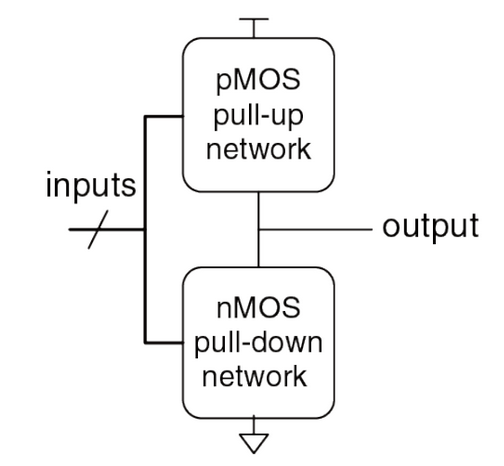
\includegraphics[width=\textwidth]{images/general_cmos_element_scheme.png}
    \caption{Общий принцип построения схем в CMOS логике}
    \label{fig:cmos_general}
\end{figure}
\FloatBarrier

В качестве элементарных частиц используем $NOT, NAND, NOR$ (нельзя сделать $AND$ и $OR$ эффективнее, чем соответствующий $NAND/NOR \circ NOT$)

Fun Fact: можно сделать $NOR$ и $NAND$ на много входов эффективнее, чем просто внешне композировать (например, для трёх — 6 вместо 8-и).


\subsubsection{Дребезг контактов}

Кнопки из реальной жизни при нажатии не сразу устанавливается в новой состояние, а сначала колеблется. 
Это назвается Contact bounce (дребезг контактов). Причём чем старше и некачественнее контакты, тем дольше будет происходить bouncing.

Есть несколько подходов к борьбе с ним. Бывает, программно, бывает аппаратно.
Причём криме вопросов реализации возникают ещё и концептуальные. 
Проще всего реагировать на нажатие с запозданием: по истечении времени с начала или с последнего изменения.
Другой вариант — реагировать как только произошло изменение после затишья, но после этого игнорировать дребезг, пока не установится.
Однако, если у нас не просто бинарная кнопка с одним контактом «нажат/не нажат», 
а имеющая положения «не нажата, положение 1 и положение 2» и мы хотим на выход подавать бинарный сигнал в виде последнего «ка\'санного» контакта, 
то всё гораздо очевиднее и у нас есть ультимативное решение через триггер и, возможно, транзистор.
Не забыть про подтягивающие резисторы.




\subsection{Оперативная память: статическая/динамическая, организация.}

Папмять располагают в 2D решётчатой структуре.

Количество проводов $\propto cols + rows  \Rightarrow O(\sqrt{memory\_size})$

$Row$ отвечает за выбор ряда. Если он ноль, ячейка вообще не работает.

Если подаётся $true$, ячейка открывается. Можно считывать информацию с соответствующих $Col$ и $\overline{Col}$.
Также можно записывать на эти входы.

Статическая память строится как 

\begin{center}
    \begin{tabular}{|| m{10em} | m{10em} | m{12em} ||} 
     \hline
     &                          \textbf{Статическая память}  & \textbf{Динамическая память} \\ [0.5ex] 
     \hline\hline
     Скорость &                 быстрая             & медленная \\ 
     \hline 
     Количество транзисторов &  Много (≈6)          & Мало (обычно один + кондерсатор) \\ 
     \hline
     Надёжность &  Наличествует          & Постоянно дегенерирует $\Rightarrow$ надо регенерировать  \\
     \hline
     Примеры &  Регистры, кэш          & Оперативная память, видеопамять  \\
     \hline
    \end{tabular}
\end{center}

Параметры, по которым оценивается память:
\begin{center}
    Объём, 
    
    скорость доступа («latency»), 
    
    скорость передачи («throughput», пропускная способность)
\end{center}



\end{document}